\documentclass{beamer}
\mode<presentation> 
{
	\usetheme[alternativetitlepage]{Torino}
	\usecolortheme{chameleon}
	\setbeamercovered{transparent}	
}
\definecolor{olive}{RGB}{51, 149, 48}
\definecolor{red}{RGB}{195, 2, 36}

\usepackage{ucs}
\usepackage[utf8x]{inputenc}
\usepackage[czech]{babel}
\usepackage{palatino}
\usepackage{graphicx}
\usepackage{epstopdf}
\usepackage{color}
\usepackage[export]{adjustbox}
\usepackage{multicol}
\usepackage{hyperref}
\usepackage[labelfont={color=olive,scriptsize}]{caption}
\usepackage{subcaption}
\usepackage{amsmath}



\title{\large{\textbf{Detekce hran s využitím dynamického programování}}}

\author{Pavel Macenauer \\ \tiny{xmacen02@stud.fit.vutbr.cz} \\ \normalsize{Jan Bureš} \\ \tiny{xbures19@stud.fit.vutbr.cz}}
\date{\tiny{\today}}
\institute[FIT VUTBR]
{
	\inst{}
	Fakulta Informačních Technologií \\
	Vysoké Učení Technické v Brně
}

\begin{document}

	\begin{frame}[t,plain]
	\titlepage

	\vspace{-7mm}
	\center{ 
\includegraphics[height=7mm]{logo.eps} }
	\end{frame}

%% ------------- princip -------------

	\begin{frame}[t,fragile]
		\frametitle{DP a detekce hran}	
	\centering{		
	\begin{figure}[h!]	
	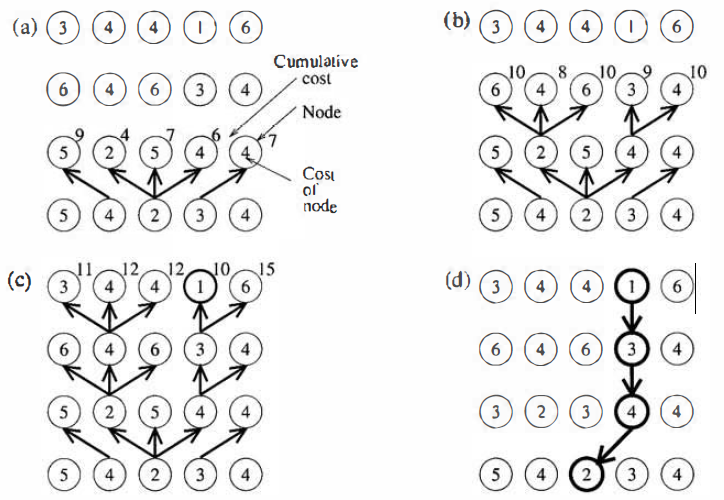
\includegraphics[height=55mm]{theory.png}	
		\end{figure}}
	\end{frame}
	
	%% ------------- princip(2) -------------

	\begin{frame}[t,fragile]
		\frametitle{DP a detekce hran}	
Postup je znázorněn odzdola nahoru, ale je možné postupovat jakýmkoliv jiným směrem. Danému řádku/sloupci budeme říkat úroveň.

		\begin{enumerate}
			\item Pro každý uzel (pixel) obrazu se spočítá ohodnocení pomocí vhodné funkce
			\item Pro každý uzel na dané úrovní vybereme jeho předchůdce a přičteme ohodnocení předchůdce k ohodnocení daného uzlu. Předchůdce se vybírá jako uzel s nejnižším ohodnocením ze sousedních pixelů v předchozí úrovni. Dostáváme akumulovanou cenu.
			\item Na poslední úrovní vybereme nejnižší akumulovanou cenu a sledováním předchůdců dostaneme optimální cestu (hranu).
		\end{enumerate}
	\end{frame}
	
	
	
		%% ------------- princip() -------------

	\begin{frame}[t,fragile]
		\frametitle{Bellmanův princip optimality}	

		Zbývající část optimální strategie je rovněž optimální, pokud proces začíná ve stavu, do kterého se dostal v důsledku použití optimální strategie.
			
		\begin{center}		
	\begin{figure}[h!]
	

	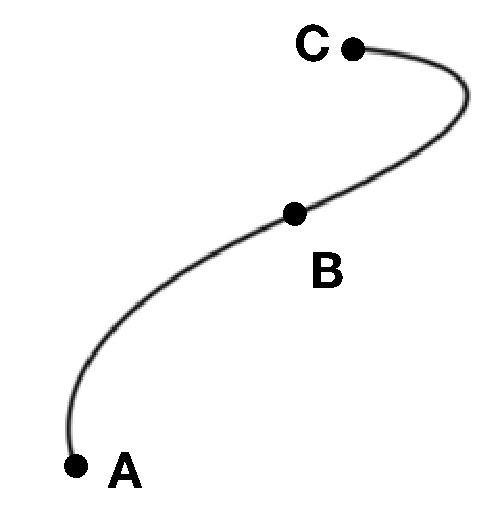
\includegraphics[height=33mm]{bellman-opt.pdf}
	\caption{\scriptsize{Je-li cesta z \textbf{A} do \textbf{C} optimální, pak existuje i cesta z \textbf{B} do \textbf{C}}}
		\end{figure}					  		
		\end{center}
	\end{frame}
	
	
	\begin{frame}[t,fragile]
		\frametitle{Využití a na co se to hodí}	

		\begin{itemize}
			\item \textbf{Hrany podlouhlých objektů} - hor, řek
			\item \textbf{Zdravotnictví} - cévy, tepny, páteř
			\item \textbf{Segmentace} - obraz je procházen od počáteční do koncové souřadnice, např. při průchodu z jednoho pixelu koncové vrstvy do pixelu první vrstvy rozdělíme obraz na 2 části podle nějaké hrany, která je cestou mezi těmito dvěma body
			\item \textbf{Výpočetní jednoduchost} - je třeba spočítat pouze ohodnocení všech uzlů a určit jejich předky, následně už samotný průchod je lineární
		\end{itemize}
		
	\end{frame}
	
	\begin{frame}[t,fragile]
		\frametitle{Vyhodnocování uzlů}	

		$$ E_{sum} = C_{discont}E_{discont}(p_{i-1},p_{i})-C_{int}E_{int}(p_{i})-C_{grad}E_{grad}(p_{i}) $$
		
		$E$ \ldots jednotlivé cenové funkce \\
		$C$ \ldots váhy pro dané funkce \\
		$p_{i}$ \ldots pixel
		
		\vspace{5mm}\centering
		\begin{tabular}{lll}
			\vspace{-5mm}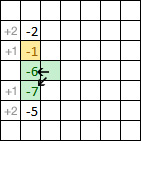
\includegraphics[height=30mm]{disc.jpg} &		
			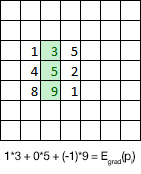
\includegraphics[height=30mm]{grad.jpg} &
			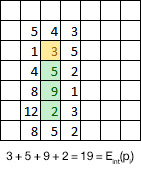
\includegraphics[height=30mm]{int.jpg}
		\end{tabular}
		

	\end{frame}
	
	\begin{frame}[t,fragile]
		\frametitle{Cenové funkce}	
\centering	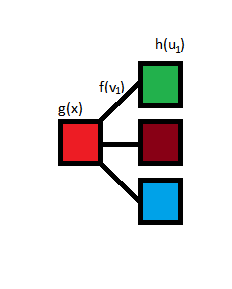
\includegraphics[height=38mm]{cenovefce.png}
\vspace{-5mm}
	\begin{itemize}
		\item \textbf{rozdíl RGB složek} - rozdíl jednotlivých barevných složek 2 sousedních pixelů a následný součet
		\item \textbf{rozdíl CMYK složek} - stejné jako RGB, pouze s převodem na CMYK
		\item \textbf{rozdíl odstínů šedé} - stejné jako RGB, pouze s převodem na odstíny šedé
	\end{itemize}
		
	\end{frame}
	
	\begin{frame}[t,fragile]
		\frametitle{Hledání cest v polárním prostoru}	

\centering{
	\begin{tabular}{ll}
			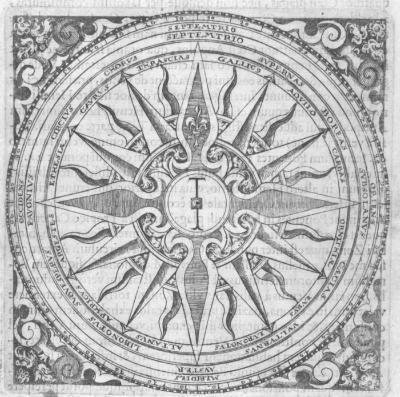
\includegraphics[height=30mm]{polar2.jpg} &		
			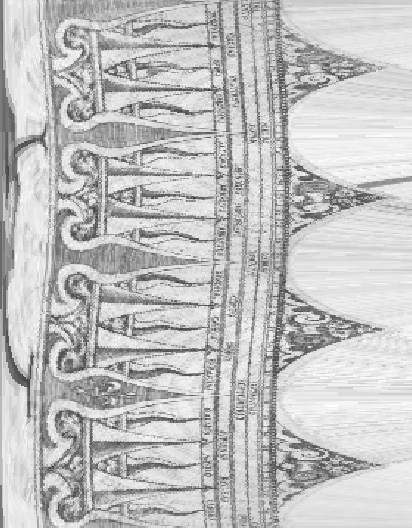
\includegraphics[height=30mm]{polar.jpg}
		\end{tabular}		}
		
		\begin{itemize}
\item kulaté objekty jsou v polárním prostoru lineární, je tak jednodušší detekovat hranu
\item implementace pomocí lookup tabulky souřadnic
\begin{itemize}
\item vytvoří se polární kopie obrazu z kartézského
\item do tabulky se zapíše jaký polární bod odpovídá jakému kartézskému
\item provede se detekce hran
\item podle tabulky se zpětně zjistí odpovídající body
\end{itemize}
\end{itemize}
	\end{frame}
	
	\begin{frame}[t,fragile]
		\frametitle{Výsledky lineární detekce hran}	
\begin{center}


		\begin{tabular}{lll}
			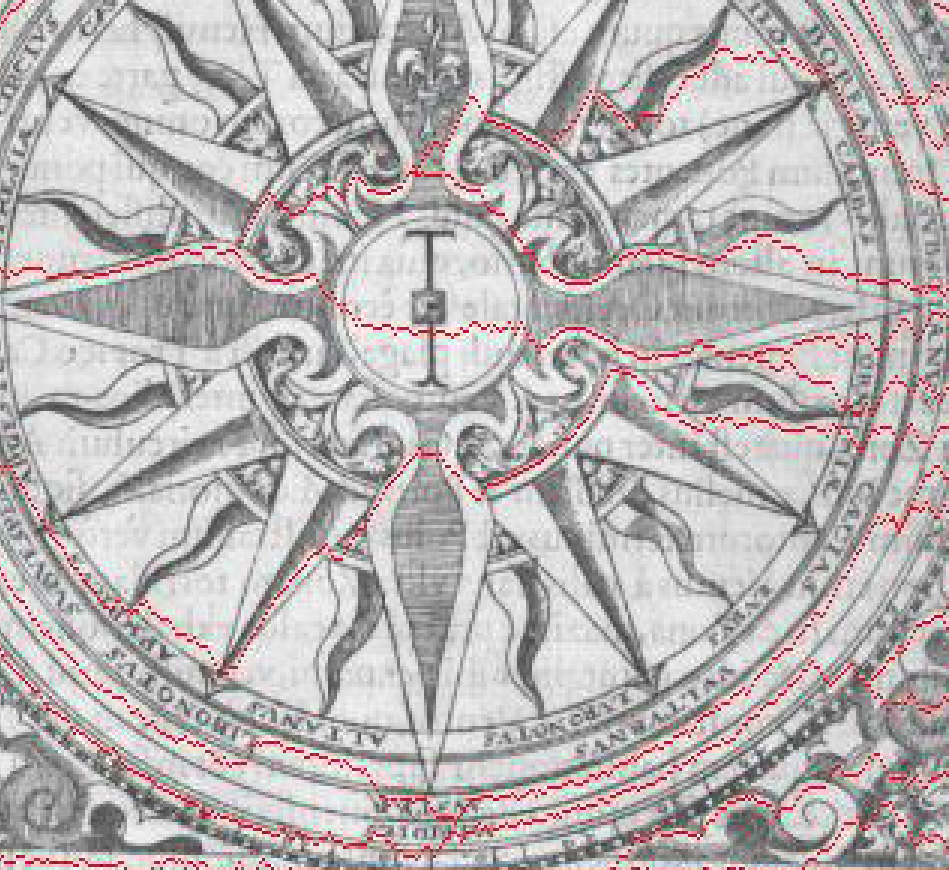
\includegraphics[height=33mm]{300p-res.jpg} &		
			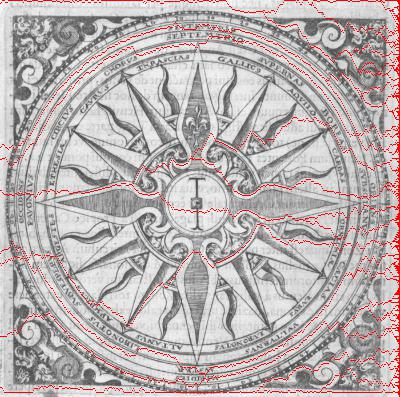
\includegraphics[height=33mm]{res-left-right.jpg} &
			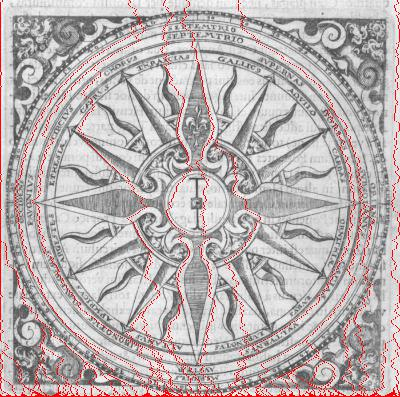
\includegraphics[height=33mm]{res-top-bottom.jpg}
		\end{tabular}		
	\end{center}	
	
		
\centering{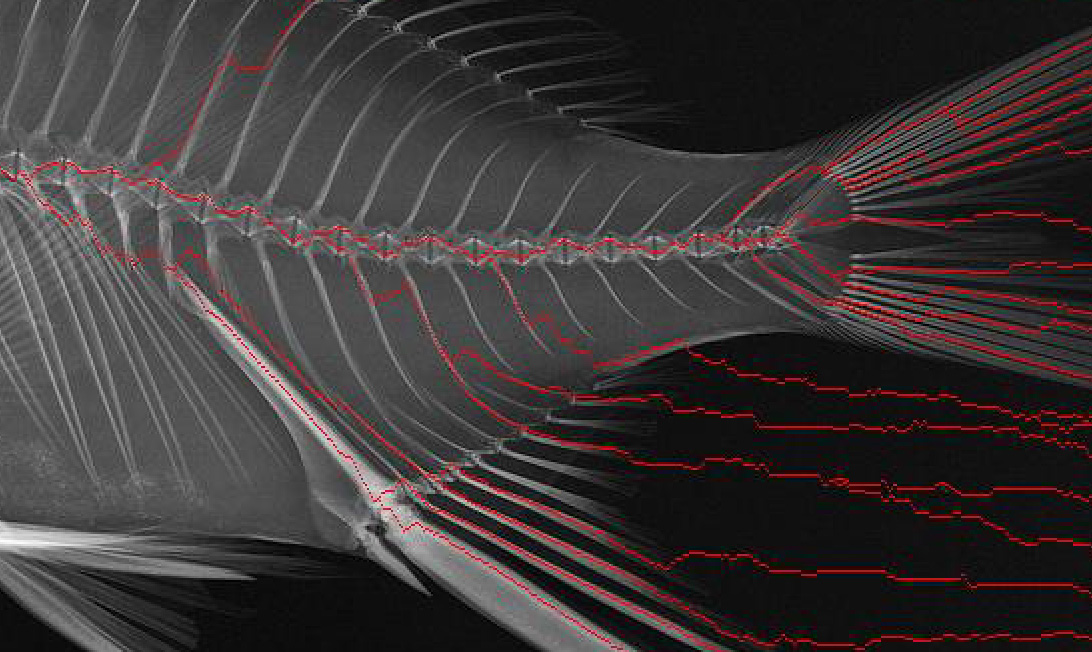
\includegraphics[height=27mm]{fish.jpg}}
		
	\end{frame}
	

	
	\begin{frame}[t,fragile]
		\frametitle{Výsledky polární detekce hran}	
\begin{center}


		\begin{tabular}{ll}
			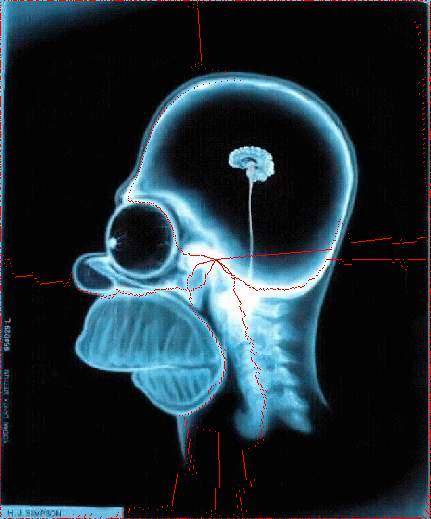
\includegraphics[height=60mm]{homer-polar.jpg} &		
			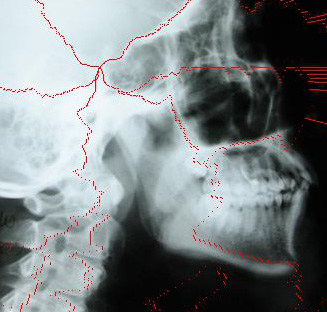
\includegraphics[height=50mm]{skull.jpg}
		\end{tabular}
		\end{center}
	
		

		
	\end{frame}
	
\end{document} 
